\section{Simplified Model}

\subsection{Steady States}

In this section I will handled the simplified model, so I could check
my numerical simulation. The model is:

\begin{align*}
b_{t} & =G_{b}b\left(1-b\right)-b+\delta_{b}\nabla^{2}b\\
w_{t} & =p-\nu w-G_{w}w+\delta_{w}\nabla^{2}w\\
G_{b} & =\nu w\left(1+\eta b\right)^{2}\\
G_{w} & =\gamma b\left(1+\eta b\right)^{2}
\end{align*}

We want to find stable constant states:

\begin{align*}
\nu w\left(1+\eta b\right)^{2}b\left(1-b\right)-b & =0\\
p-\nu w-\gamma b\left(1+\eta b\right)^{2}w & =0\\
\Rightarrow w & =\frac{p}{\nu+\gamma b\left(1+\eta b\right)^{2}}
\end{align*}

Plugging the result into $b$ we get:

\begin{align*}
\nu\frac{p}{\nu+\gamma b\left(1+\eta b\right)^{2}}\left(1+\eta b\right)^{2}b\left(1-b\right)-b & =0
\end{align*}

We can see that $b=0,w=\frac{p}{\nu}$ is one stable solution. If
$b\neq0$ then the other solutions can be found by numerical methods.
We need to find the roots of

\begin{align*}
G_{b}\left(1-b\right)-1 & =0\\
p-\nu w-G_{w}w & =0
\end{align*}

Plotting the numerical results against $p$ we get:

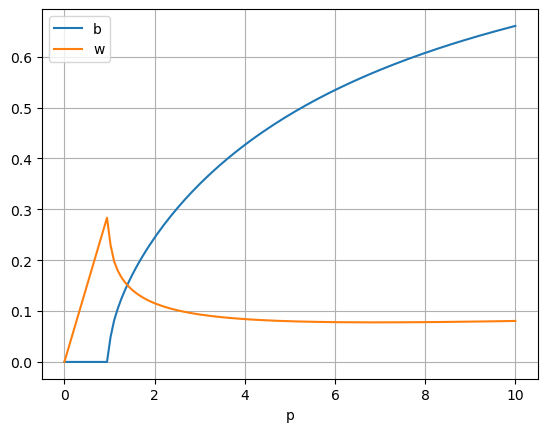
\includegraphics[scale=0.5]{plots/pasted1.png}

\subsection{Linear Stability Analysis - Uniform Perturbation}

For a uniform perturbation all the $\nabla^{2}$ terms are zero. The
equation then becomes:

\begin{align*}
\left[\begin{array}{c}
b_{t}\\
w_{t}
\end{array}\right] & =\left[\begin{array}{c}
G_{b}b\left(1-b\right)-b\\
p-\nu w-G_{w}w
\end{array}\right]=F\left(b,w\right)\\
F\left(b,w\right) & =\left[\begin{array}{c}
\nu w\left(1+\eta b\right)^{2}b\left(1-b\right)-b\\
p-\nu w-\gamma b\left(1+\eta b\right)^{2}w
\end{array}\right]
\end{align*}

We are interested in the stability of the bare soil solution ($b=0\Rightarrow w=\frac{p}{\nu}$)

\begin{align*}
\left.\frac{\partial F_{b}}{\partial b}\right|_{b=0,w=\frac{p}{\nu}} & =vw-1=p-1\\
\left.\frac{\partial F_{b}}{\partial w}\right|_{b=0,w=\frac{p}{\nu}} & =0\\
\left.\frac{\partial F_{w}}{\partial b}\right|_{b=0,w=\frac{p}{\nu}} & =-\gamma w=-\frac{\gamma}{\nu}p\\
\left.\frac{\partial F_{w}}{\partial w}\right|_{b=0,w=\frac{p}{\nu}} & =-\nu\\
\Rightarrow J & =\left[\begin{array}{cc}
p-1 & 0\\
-\frac{\gamma}{\nu}p & -\nu
\end{array}\right]
\end{align*}

Now, we find the eigenvalues

\begin{align*}
\left|J-\sigma I\right| & =\left|\begin{array}{cc}
p-1-\sigma & 0\\
-\frac{\gamma}{\nu}p & -\nu-\sigma
\end{array}\right|\\
 & =-\nu p-\sigma p+\nu+\sigma+\sigma^{2}\\
 & =\sigma^{2}+\left(1-p\right)\sigma+\left(1-p\right)\nu=0\\
\sigma & =\frac{p-1}{2}\pm\sqrt{\left(\frac{1-p}{4}\right)^{2}-\left(1-p\right)}
\end{align*}

For $p=1$ we can see the $\sigma=0$. For $0<p<1$ the discriminant
is negative, and $\frac{p-1}{2}<0\Rightarrow p<1$ so it is a stable
state. For $p>1$ there exists a mode $\sigma_{+}$ that grows so
it is an unable state (Hopf Bifurcation)

\subsection{Variational Formulation}

To use the FEniCS library, a variational formulation is needed for
the model

\begin{align*}
b_{t} & =G_{b}b\left(1-b\right)-b+\delta_{b}\nabla^{2}b\\
w_{t} & =p-\nu w-G_{w}w+\delta_{w}\nabla^{2}w\\
G_{b} & =\nu w\left(1+\eta b\right)^{2}\\
G_{w} & =\gamma b\left(1+\eta b\right)^{2}
\end{align*}
 with periodic boundary conditions.

\begin{align*}
\left\langle \frac{b-b^{n}}{\Delta t},v_{1}\right\rangle -\left\langle G_{b}b\left(1-b\right)-b,v_{1}\right\rangle +\delta_{b}\left\langle \nabla b,\nabla v_{1}\right\rangle \\
+\left\langle \frac{w-w^{n}}{\Delta t},v_{2}\right\rangle -\left\langle p-\nu w-G_{w}w,v_{2}\right\rangle +\delta_{w}\left\langle \nabla w,\nabla v_{2}\right\rangle  & =0
\end{align*}

with
\begin{align*}
G_{b} & =\nu w\left(1+\eta b\right)^{2}\\
G_{w} & =\gamma b\left(1+\eta b\right)^{2}
\end{align*}

The constants in the simulation are:

\begin{align*}
\nu & =\frac{10}{3}\\
\gamma & =\frac{50}{3}\\
\eta & =3.5\\
\delta_{b} & =\frac{1}{30}\\
\delta_{w} & =\frac{10}{3}
\end{align*}
